\documentclass[a4paper, 12pt]{article}

\usepackage[english,russian]{babel}
\usepackage[T2A]{fontenc}
\usepackage[utf8]{inputenc}
\usepackage{geometry}
\usepackage{enumitem}
\usepackage{setspace}
\usepackage{amssymb}
\usepackage{graphicx}
\usepackage{wrapfig}
\usepackage{float}
\usepackage{amsmath}
\usepackage{textcomp}
\usepackage{dsfont}

\geometry{top=5mm, left=1cm}
%\setlength{\parindent}{0}
\renewcommand{\arraystretch}{1.2}
\linespread{1}

\begin{document}
    \begin{center}
        \textbf{Сферическая геометрия №3}\\
        Расстояние между точками, углы между прямыми, сферические окружности.
    \end{center}

    \begin{center}
        \textbf{№ 1}
    \end{center}

    Докажите, что сумма смежных углов между сферическими прямыми равна $180^\circ$

    \textbf{Решение}\\

    \begin{center}
        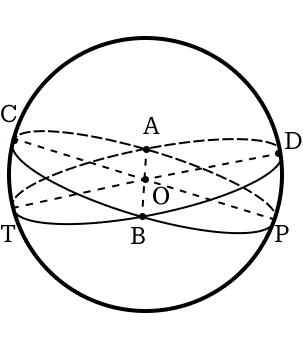
\includegraphics[width=0.2\textwidth]{images/img4}\\
    \end{center}

    1) $\angle TOC = \angle TBC$, $\angle COD = \angle CBD$ как линейные углы.

    2) $\angle TOC$ и $\angle COD$ - смежные в плоскости $(TOC)$, тогда $\angle TOC + \angle COD = 180^{\circ}$

    3) Таким образом,
    \[
        \angle TOC + \angle COD = 180^{\circ} = \angle TBCC + \angle CBD \text{ - что и требовалось доказать.}
    \]

    \begin{center}
        \textbf{№ 2}
    \end{center}

    Докажите, что вертикальные углы между сферическими прямыми равны

    \textbf{Решение}\\

    \begin{center}
        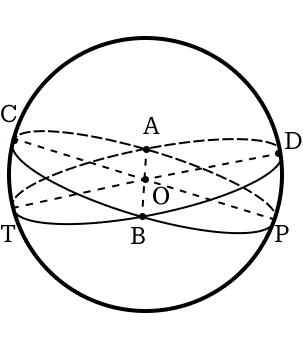
\includegraphics[width=0.2\textwidth]{images/img5}\\
    \end{center}

    1) $\angle TOC = \angle TBC$, $\angle POD = \angle PBD$ как линейные углы.

    2) $\angle TOC = \angle POD$ как вертикальные углы в плоскости $(TOP)$.

    3) Таким образом:
    \[
        \angle TOC = \angle POD = \angle TBC = \angle PBD \text{ - что и требовалось доказать.}
    \]

    \begin{center}
        \textbf{№ 3}
    \end{center}

    Радиус сферы равен $R$, евклидово расстояние между двумя точками сферы равно $h$,
    чему равно сферическое расстояние между этими точками.

    \textbf{Решение}\\

    \begin{center}
        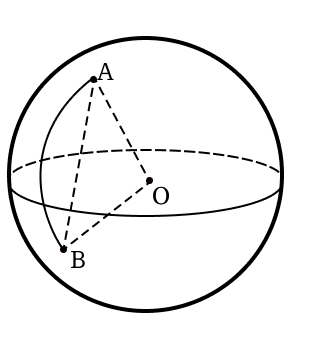
\includegraphics[width=0.2\textwidth]{images/img6}\\
    \end{center}

    1) $AO = BO = R$, $AB = h$

    2) По теореме косинусов:
    \[
        AB ^ 2 = OB ^ 2 + OA ^ 2 - 2OB*OA*\cos BOA
    \]
    \[
        \cos BOA = -\frac{AB^2 - OB^2 - OA^2}{2OB*OA} = -\frac{h^2 - 2R^2}{2R^2} = 1 - \frac{h^2}{2r^2}
    \]
    \[
        \angle BOA = \arccos \left(1 - \frac{h^2}{2r^2}\right)
    \]

    3)
    \[
        \cup AB = R\angle BOA = R \arccos \left(1 - \frac{h^2}{2r^2}\right)
    \]

    Ответ: $R \arccos \left(1 - \frac{h^2}{2r^2}\right)$

    \begin{center}
        \textbf{№ 4}
    \end{center}

    На большой окружности отметили две точки и провели к ним радиусы.
    Чему равно сферическое и евклидово расстояние между этими точками, если радиус сферы равен 13 см,
    а угол между радиусами равен $\frac{\pi}{6}$.

    \textbf{Решение}\\

    \begin{center}
        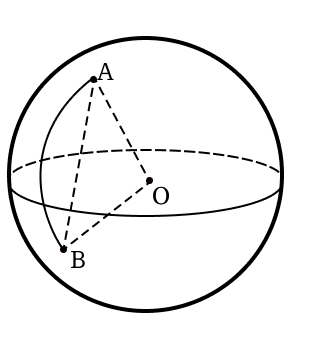
\includegraphics[width=0.2\textwidth]{images/img7}\\
    \end{center}

    1)
    \[
        \cup AB = 13 * \frac{\pi}{6} \text{ см}
    \]

    2) По теореме косинусов:
    \[
        AB ^ 2 = AO ^ 2 + BO ^ 2 - 2AO*BO*\cos BOA = 2 * 169 - 2 * 169 * \frac{\sqrt {3}}{2} = 169(2 - \sqrt {3}) \text{ см}^2
    \]
    \[
        AB = 13\sqrt {2 - \sqrt {3}} \text{ см}
    \]\\

    Ответ: $\cup AB = 13\frac{\pi}{6}$ см, $AB = 13\sqrt {2 - \sqrt {3}}$ см.
    \begin{center}
        \textbf{№ 5}
    \end{center}

    Угол между двумя сферическими прямыми равен $\frac{\pi}{4}$, радиус сферы равен $7$ см.
    Из центра сферы в плоскостях сечений восстановили перпендикуляры так, что получилось 4 точки пересечения со сферой.
    Найдите сферическое расстояние между всеми этими точками.

    \textbf{Решение}\\

    \begin{center}
        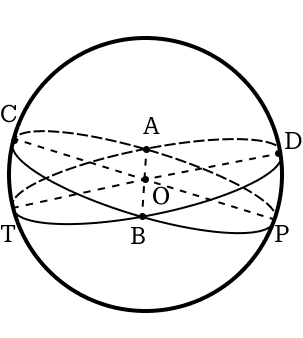
\includegraphics[width=0.2\textwidth]{images/img8}\\
    \end{center}

    1) $\angle TOC = \frac{\pi}{4}$, $TO = CO = PO = DO = 7$ см.

    2)
    \[
        \cup CT = \cup PD = 7\frac{\pi}{4} \text{ см}
    \]

    3) \[
           \cup CD = \cup TP = 7\left(\pi - \frac{\pi}{4}\right) = 7*\frac{3\pi}{4}\text{ см}
    \]

    4) \[
           \cup TD = \cup CP = 6\pi \text{ см}
    \]\\

    Ответ: $\cup CT = \cup PD = 7\frac{\pi}{4} \text{ см}; \cup CD = \cup TP = 7*\frac{3\pi}{4}\text{ см}; \cup TD = \cup CP = 6\pi \text{ см}$

    \begin{center}
        \textbf{№ 6}
    \end{center}

    На сфере радиуса $R$ построена сферическая окружность радиусом $r$.
    Чему равен радиус малой окружности, совпадающей с данной?

    \textbf{Решение}\\

    \begin{center}
        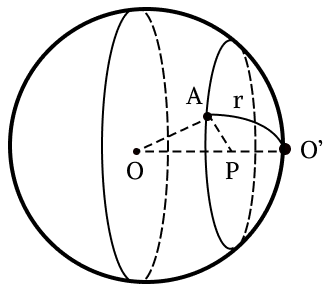
\includegraphics[width=0.2\textwidth]{images/img9}\\
    \end{center}

    1) $OO' = OA = R$, $AP \bot OO'$

    2)
    \[
        r = R*\angle O'OA \rightarrow \angle O'OA = \frac{r}{R}
    \]

    3)
    \[
        AP = OA * \sin POA = R * \sin \frac{r}{R}
    \]

    Ответ: $R\sin \frac{r}{R}$

    \begin{center}
        \textbf{№ 7}
    \end{center}

    На сфере радиуса $R$ построена сферическая окружность радиусом $r$.
    Чему равно евклидово расстояние между центром сферической окружности и центром малой окружности,
    совпадающей с данной?

     \textbf{Решение}\\

    \begin{center}
        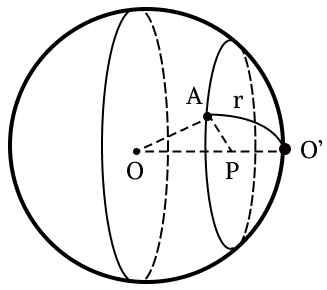
\includegraphics[width=0.2\textwidth]{images/img10}\\
    \end{center}

    1) Из задачи 6 имеем: $\angle POA = \frac{r}{R}$, тогда:
    \[
        OP = OA * \cos POA = R\cos \frac{r}{R}
    \]
    Следовательно
    \[
        PO' = OO' - OP = R - R\cos \frac{r}{R} = R\left(1 - \cos \frac{r}{R}\right)
    \]

    Ответ: $R\left(1 - \cos \frac{r}{R}\right)$

    \begin{center}
        \textbf{№ 8}
    \end{center}

    На сфере радиуса $R$ проведены три попарно перпендикулярных сферических прямых.
    Найдите периметр и площадь треугольника, образованного точками пересечения этих прямых.

    \textbf{Решение}\\

    \begin{center}
        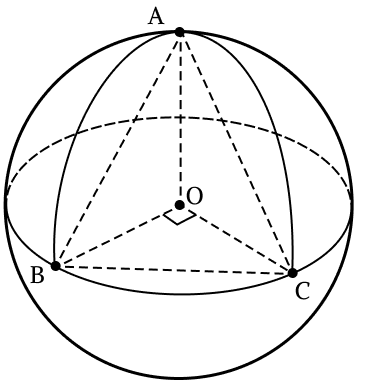
\includegraphics[width=0.2\textwidth]{images/img11}\\
    \end{center}

    1) По теореме Пифагора:
    \[
        AB = BC = AC = R\sqrt {2}
    \]

    2)\[
          P_{\triangle ABC} = 3R\sqrt {2}
    \]

    3)
    \[
        S_{\triangle ABC} = \frac{AB^2\sqrt {3}}{4} = \frac{R^2\sqrt {3}}{2}
    \]\\

    Ответ: $P_{\triangle ABC} = 3R\sqrt {2}; S_{\triangle ABC} = \frac{AB^2\sqrt {3}}{4} = \frac{R^2\sqrt {3}}{2}$


    \begin{center}
        \textbf{№ 9}
    \end{center}

    Большая и малые окружности имеют одну общую точку.
    Чему равен угол между образующими их плоскостями, если радиус сферической окружности,
    совпадающей с малой окружностью, равен $r$, а радиус сферы равен $R$.

    \textbf{Решение}\\

    \begin{center}
        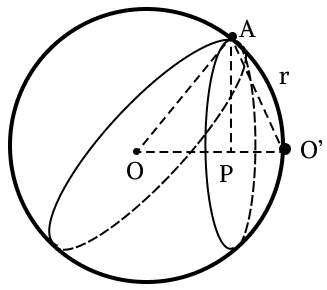
\includegraphics[width=0.2\textwidth]{images/img12}\\
    \end{center}

    1) $OP$ перпендикулярно плоскости малой окружности, тогда касательная $\alpha$, проведенная к сфере
    в плоскости большой окружности через точку $A$ перпендикулярна проведенному к ней радиусу $OA$,
    что по обратной теореме о трех перпендикулярах означает $\alpha \bot PA$, то есть $\alpha \bot (OPA)$ по признаку.
    Следовательно, $OA \bot \alpha$ и $PA \bot \alpha$, значит $\angle OAP$ - равен искомому углу.

    2)
    \[
        r = \angle AOP * R \rightarrow \angle AOP = \frac{r}{R} \rightarrow \angle OAP = \frac{\pi}{2} - \frac{r}{R}
    \]

    Ответ: $\frac{\pi}{2} - \frac{r}{R}$

    \begin{center}
        \textbf{№ 10}
    \end{center}

    Чему равно сферическое расстояние между полярно сопряженными точками, если радиус сферы равен $R$?

     \textbf{Решение}\\

    \begin{center}
        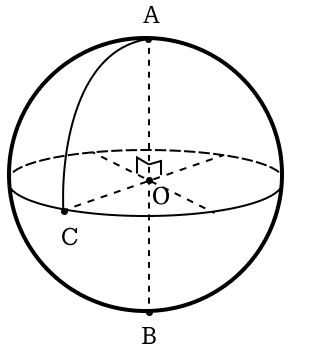
\includegraphics[width=0.2\textwidth]{images/img13}\\
    \end{center}

    1) $\angle COA = \frac{\pi}{2}$\\

    2) $\cup AC = R\frac{\pi}{2}$\\

    Ответ: $R\frac{\pi}{2}$

    \begin{center}
        \textbf{№ 11}
    \end{center}

    Проведены две сферические прямые, пересекающиеся под углом $\alpha$,
    перпендикулярно к ним проведена третья сферическая прямая.
    Чему равен радиус сферы, если сферическое расстояние между точками пересечения
    двух прямых третьей равно $h$?

    \textbf{Решение}\\

    \begin{center}
        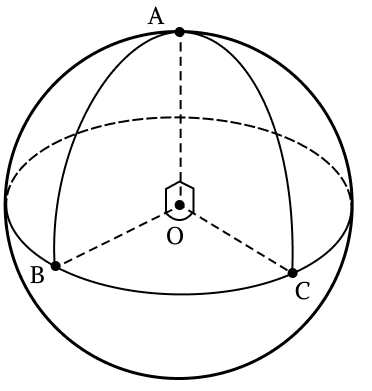
\includegraphics[width=0.2\textwidth]{images/img14}\\
    \end{center}

    1) $BC = h$, $\angle BOC = \alpha$

    2) \[
           h  = \alpha * R \rightarrow R = \frac{h}{\alpha}

    \]

    Ответ: $\frac{h}{\alpha}$
\end{document}
